\begin{frame}{\mcts{} (MCTS)}
    \begin{itemize}
        \item MCTS is a recent algorithm for {\em sequential decision making}
        \item It applies to \mdp{} (MDP)
        \begin{itemize}
            \item discrete-time $t$ with finite horizon $\horizon$
            \item state $\state_t \in \statespace$
            \item action $\decision_t \in \decisionspace$
            \item transition function $\state_{t+1} = \transitionfunction(\state_t, \decision_t)$
            \item cost function $\reward_t = \costfunction_\transitionfunction(\state_t)$
            \item reward $\globalreward = \sum_{t = 0}^{\horizon}{\reward_t}$
            \item policy function $\decision_t = \policy_{\transitionfunction}(\state_t)$
            \item we look for the policy $\policy^*$ that maximizes expected $\globalreward$ 
        \end{itemize}
    \end{itemize}
\end{frame}


\begin{frame}{MCTS strength}
    \begin{itemize}
        \item Mcts is a versatile algorithm (it does not require knowledge about the problem)
        \item especially, does not require any knowledge about the Bellman value function
        \item stable on high dimensional problems
        \item it outperforms all other algorithms on some problems (difficult games like Go, general game playing, \dots)
    \end{itemize}
\end{frame}


\begin{frame}{MCTS}
    Problems are represented as a tree structure:
    \begin{itemize}
        \item blue circles = states
        \item plain edges + red squares = decisions
        \item dashed edges = stochastic transitions between two states
    \end{itemize}
    \begin{center}
        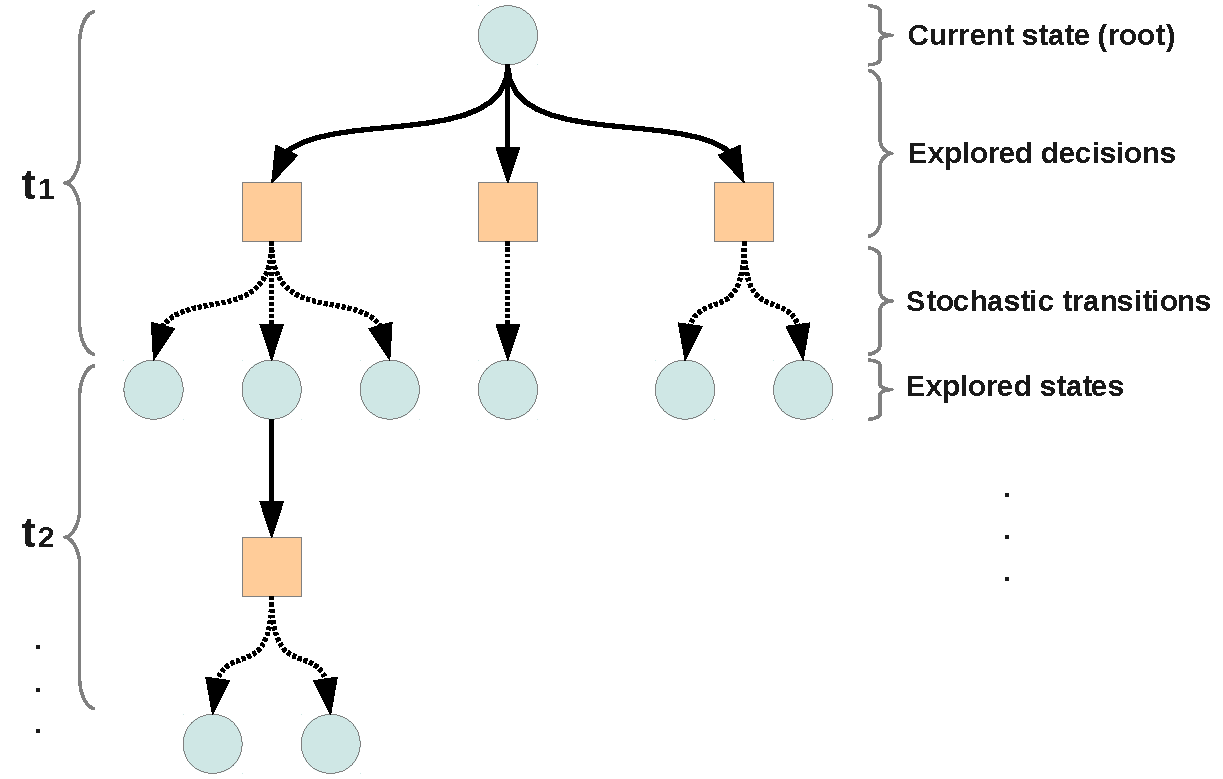
\includegraphics[width=.65\linewidth]{figs/tree}
    \end{center}
\end{frame}
